\PassOptionsToPackage{unicode}{hyperref}
\documentclass[aspectratio=1610, 9pt]{beamer}

% Load packages you need here
\usepackage{polyglossia}
\setmainlanguage{german}

\usepackage{csquotes}
\usepackage{graphicx}
\usepackage{siunitx}
\usepackage{amsmath}
\usepackage{amssymb}
\usepackage{mathtools}

\usepackage{hyperref}
\usepackage{bookmark}

% load the theme after all packages

\usetheme[
  showtotalframes, % show total number of frames in the footline
   dark, % optional dark theme, uncomment to use
]{tudo}

% Put settings here, like
\unimathsetup{
  math-style=ISO,
  bold-style=ISO,
  nabla=upright,
  partial=upright,
  mathrm=sym,
}
\begin{document}
\begin{frame}
  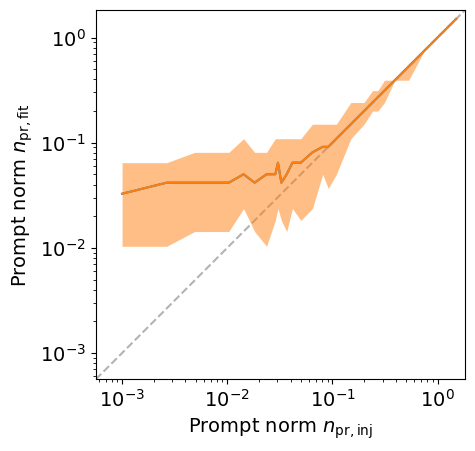
\includegraphics[width=0.6\textwidth]{~/Desktop/master_thesis/Plots/bias.png}
\end{frame}
\begin{frame}
  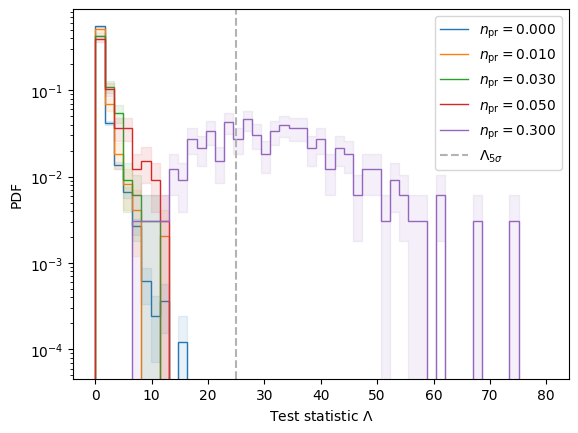
\includegraphics[width=0.7\textwidth]{../Plots/test_statistic}
\end{frame}
\begin{frame}
  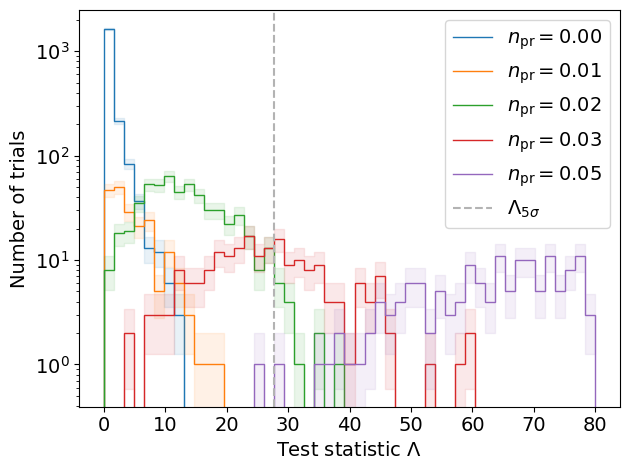
\includegraphics[width=0.7\textwidth]{../Plots/test_statisti_previous}
\end{frame}
\begin{frame}
  \frametitle{Spectra depending on cuts}
  \begin{minipage}[t]{0.24\textwidth}
    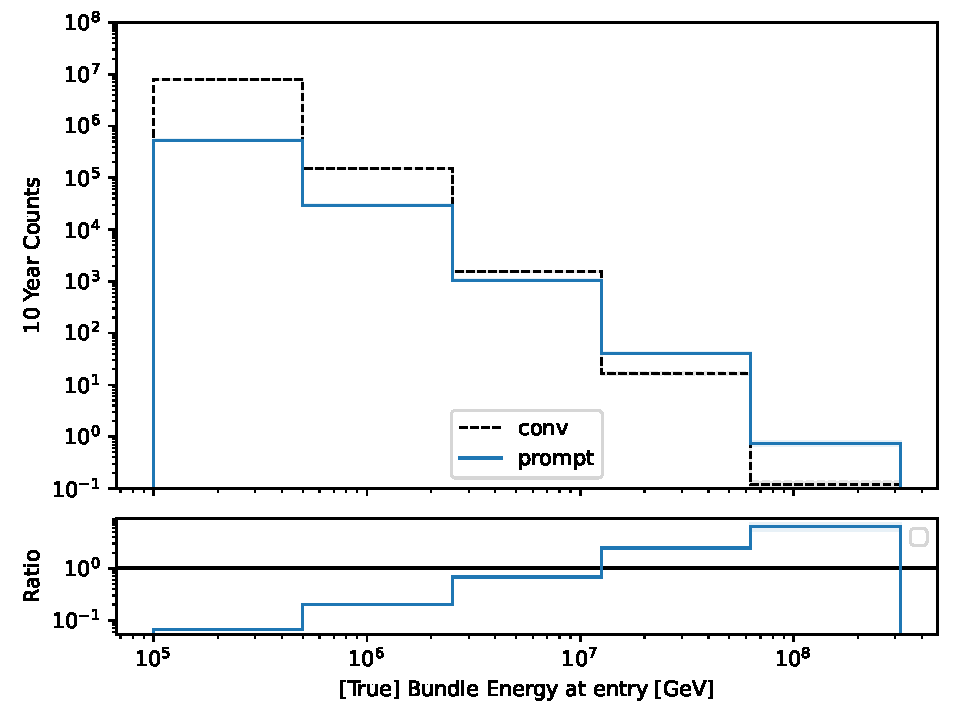
\includegraphics[width=0.85\textwidth]{../Plots/bundle_spectrum_mc.pdf}
    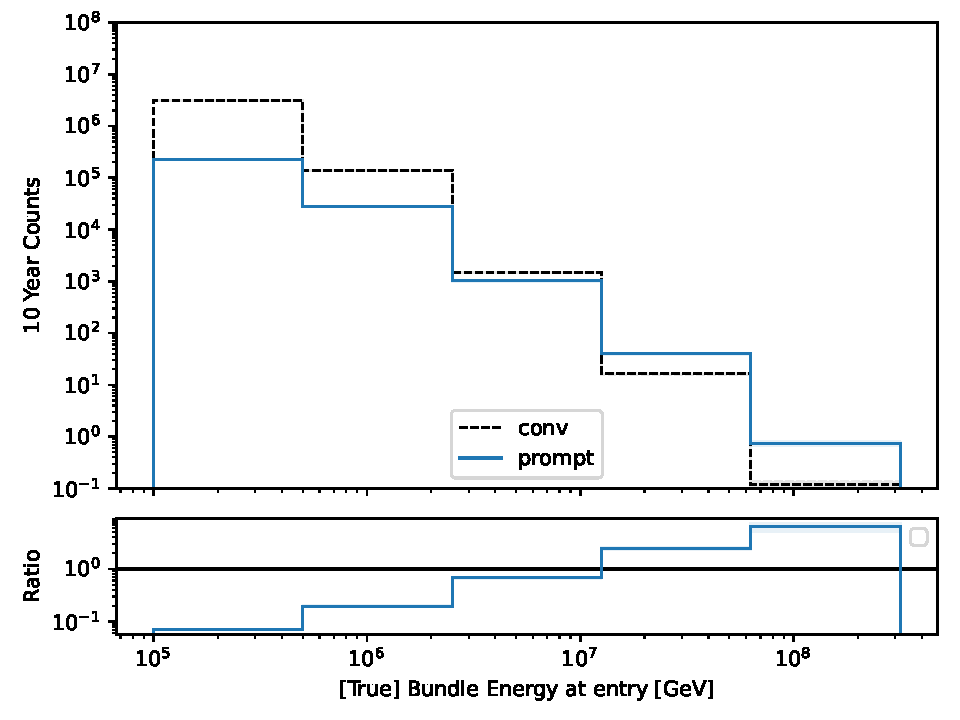
\includegraphics[width=0.85\textwidth]{../Plots/bundle_spectrum_mc_5e5surface.pdf}
    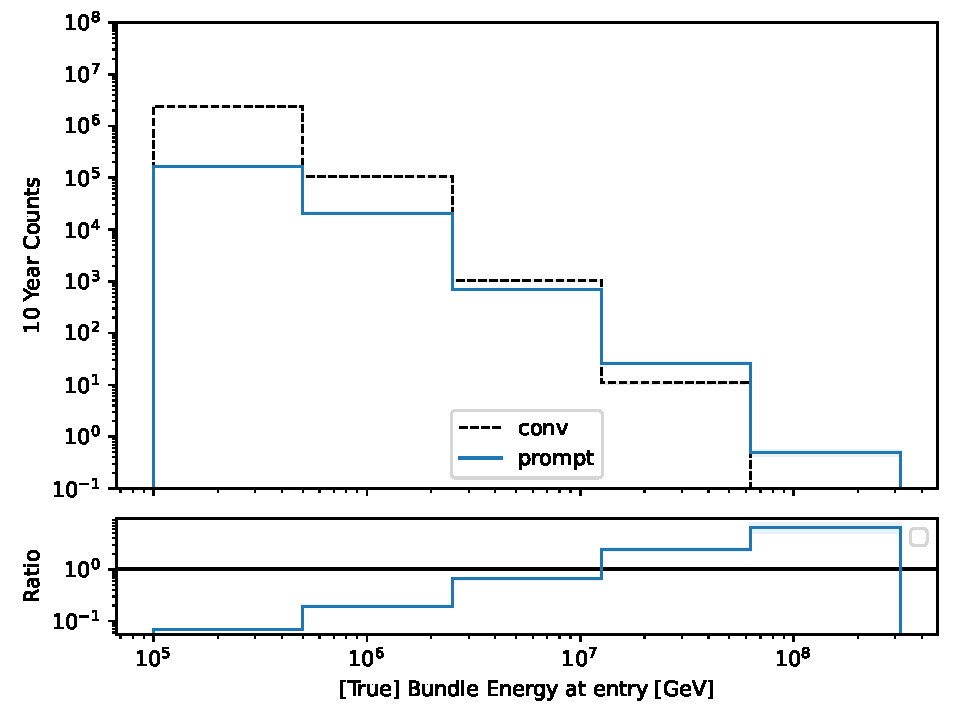
\includegraphics[width=0.85\textwidth]{../Plots/bundle_spectrum_mc_5e5surface_quality.pdf}
  \end{minipage}
  \begin{minipage}[t]{0.24\textwidth}
    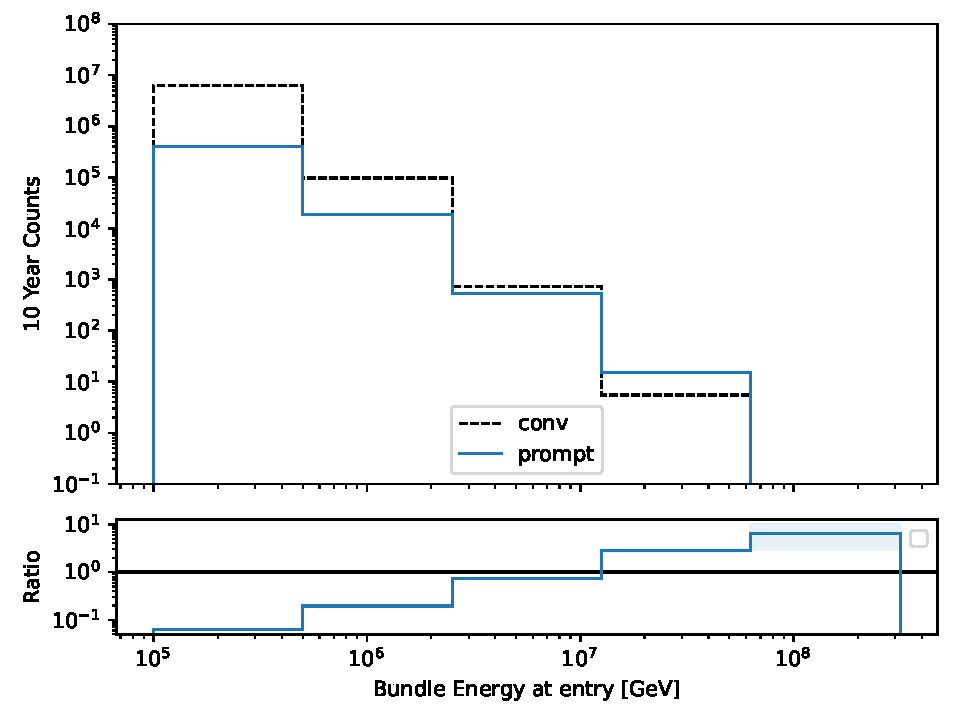
\includegraphics[width=0.85\textwidth]{../Plots/bundle_spectrum_reco.pdf}
    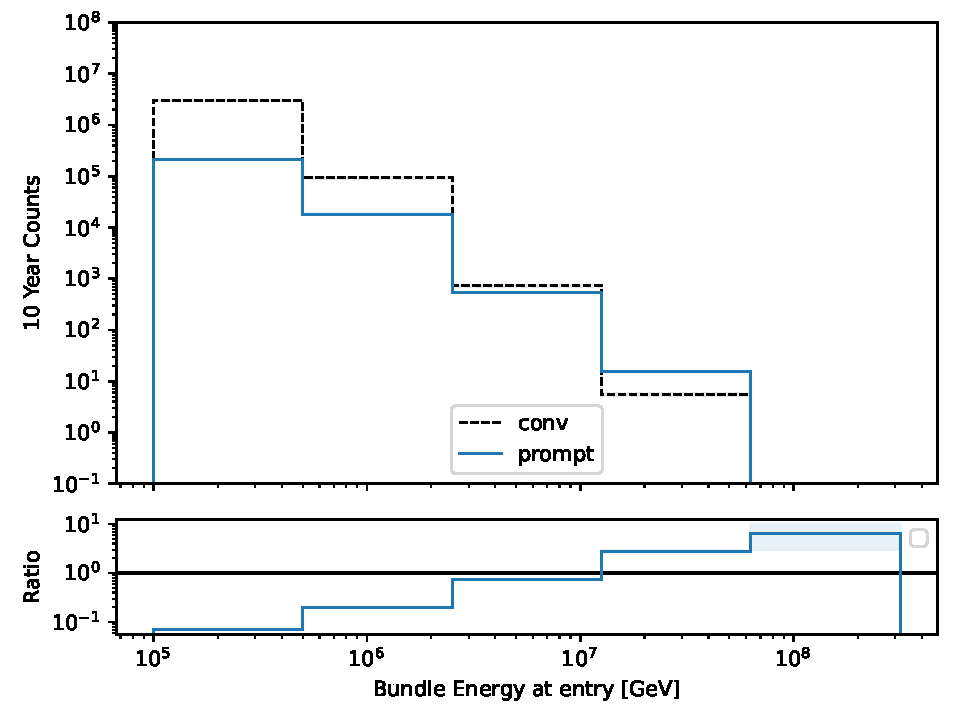
\includegraphics[width=0.85\textwidth]{../Plots/bundle_spectrum_reco_5e5_surface.pdf}
    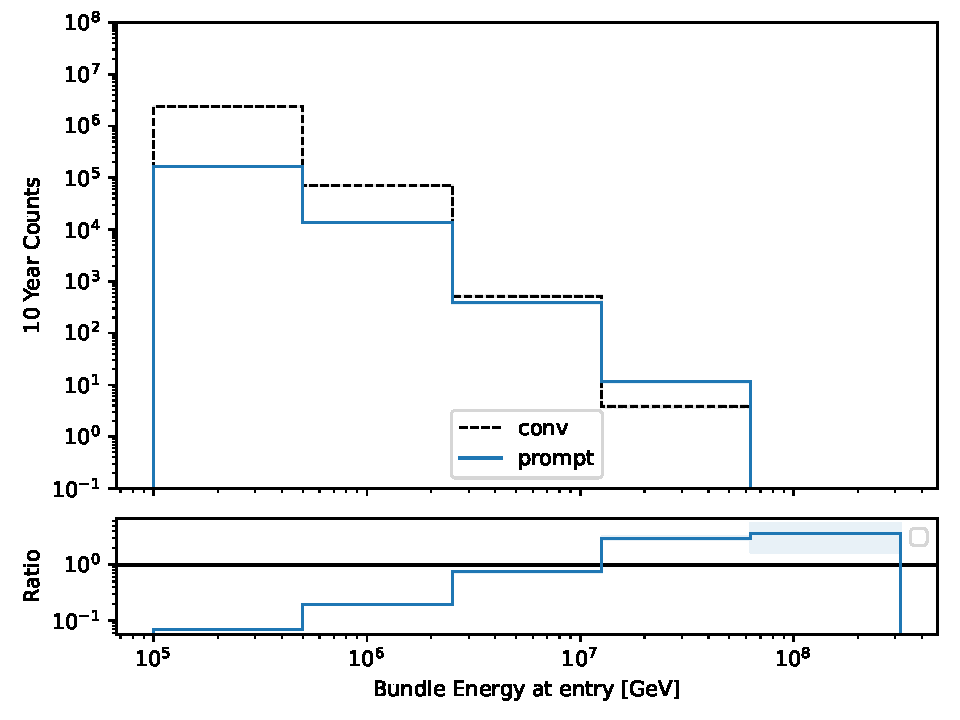
\includegraphics[width=0.85\textwidth]{../Plots/bundle_spectrum_reco_5e5surface_quality.pdf}
  \end{minipage}
  \begin{minipage}[t]{0.24\textwidth}
    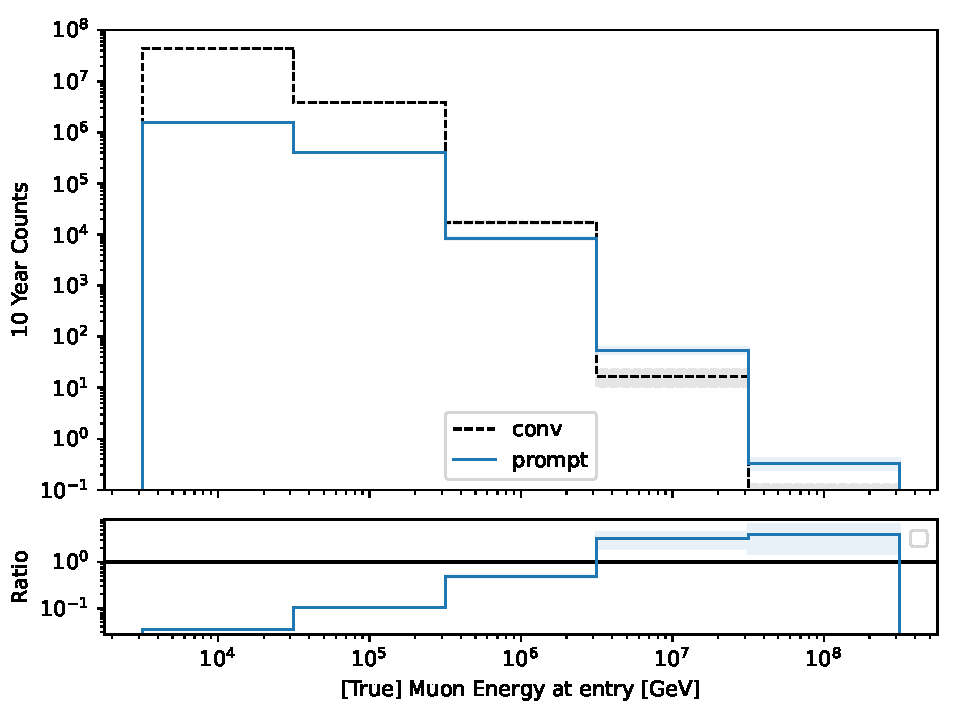
\includegraphics[width=0.85\textwidth]{../Plots/leading_spectrum_mc.pdf}
    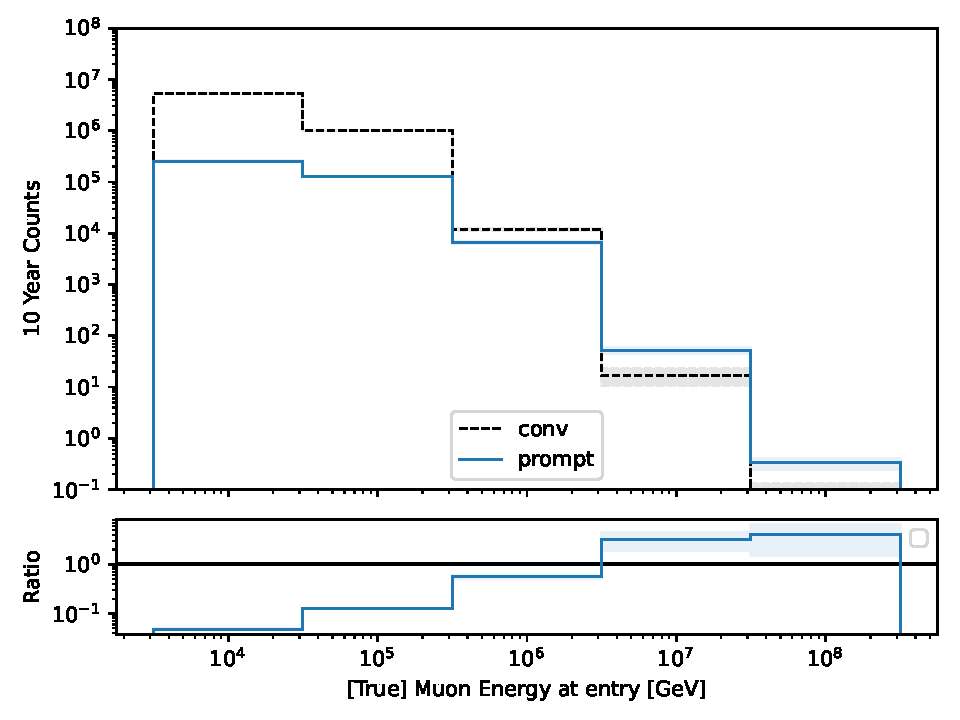
\includegraphics[width=0.85\textwidth]{../Plots/leading_spectrum_mc_5e5surface.pdf}
    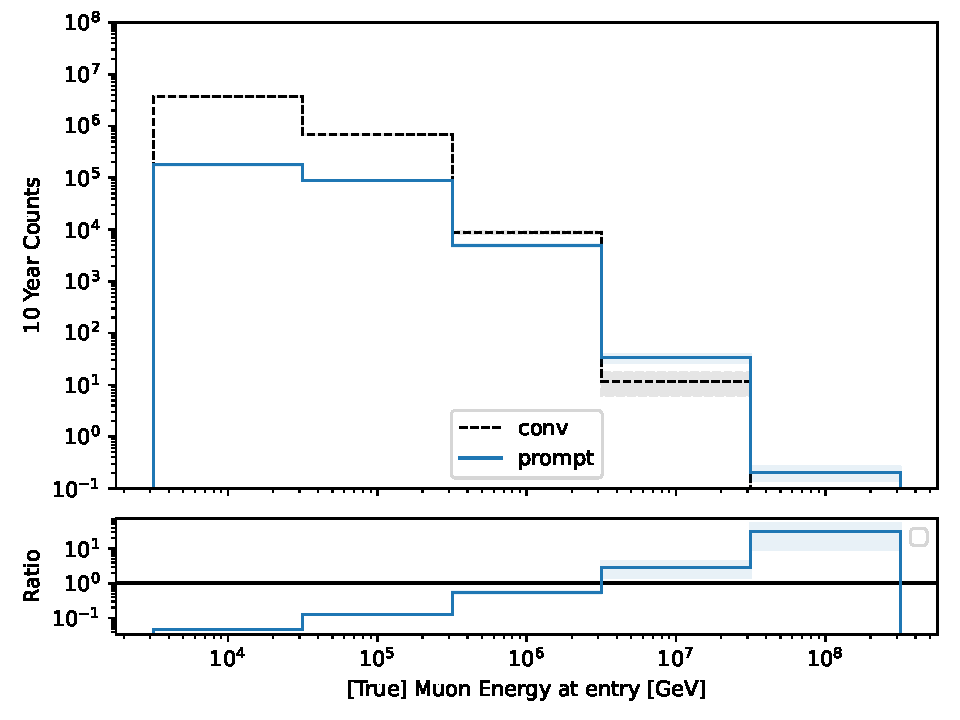
\includegraphics[width=0.85\textwidth]{../Plots/leading_spectrum_mc_5e5surface_quality.pdf}
  \end{minipage}
  \begin{minipage}[t]{0.24\textwidth}
    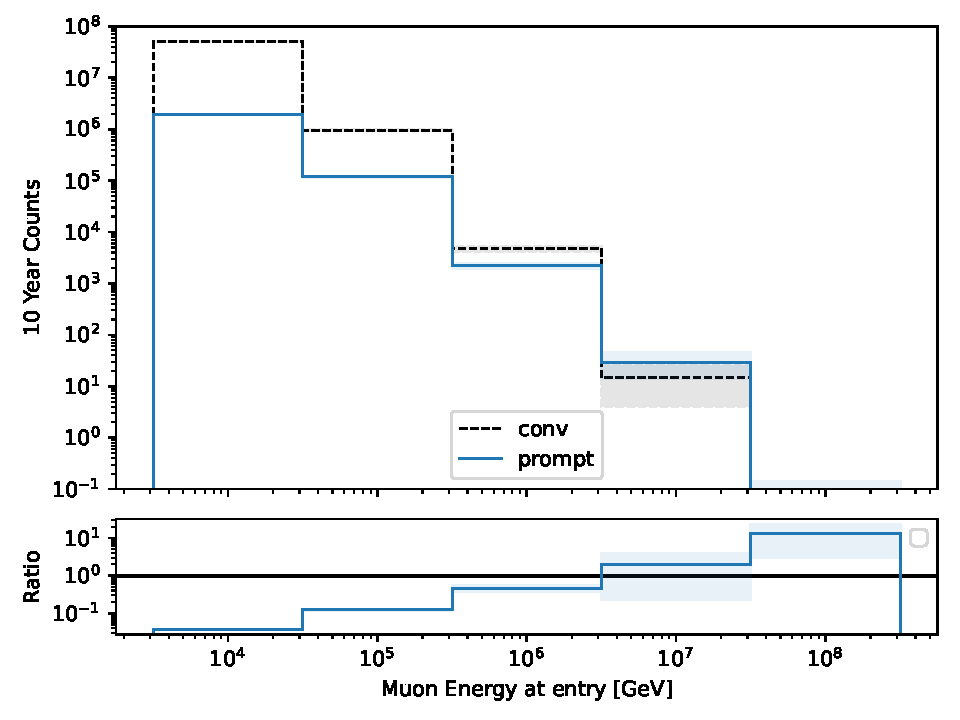
\includegraphics[width=0.85\textwidth]{../Plots/leading_spectrum_reco.pdf}
    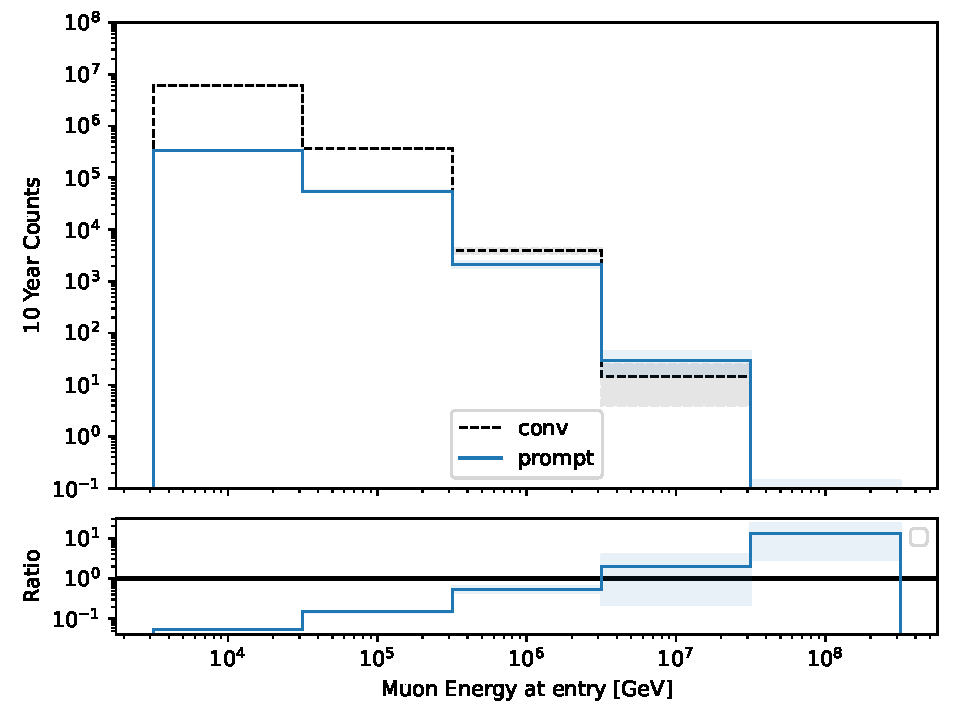
\includegraphics[width=0.85\textwidth]{../Plots/leading_spectrum_reco_5e5surface.pdf}
    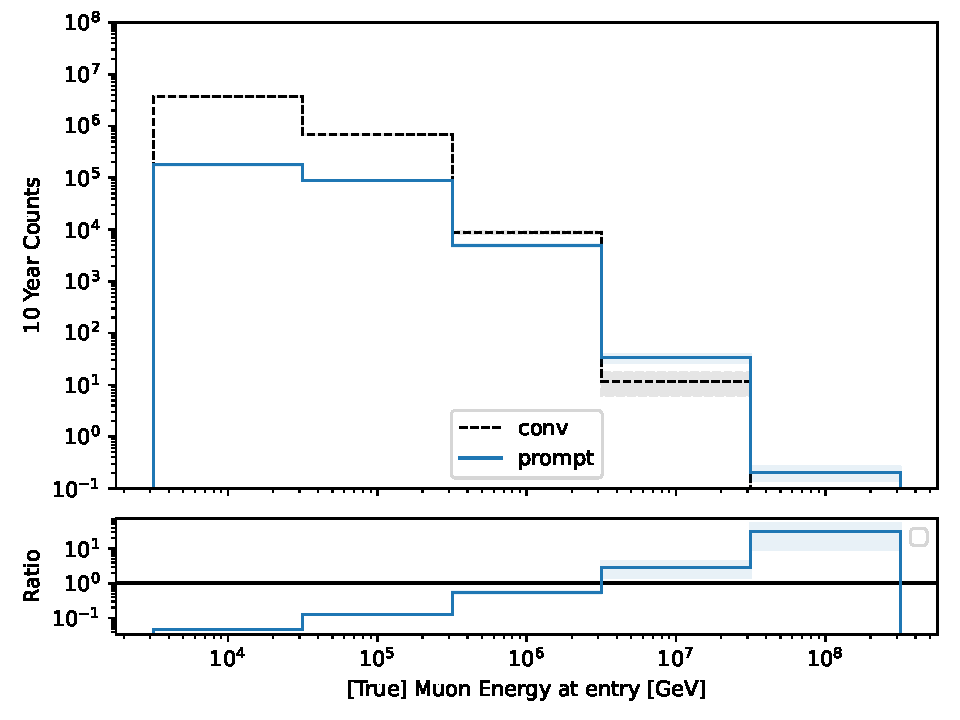
\includegraphics[width=0.85\textwidth]{../Plots/leading_spectrum_reco_5e5surface_quality.pdf}
  \end{minipage}
\end{frame}
\begin{frame}
  \frametitle{Background estimation}
  \begin{figure}
    \centering
    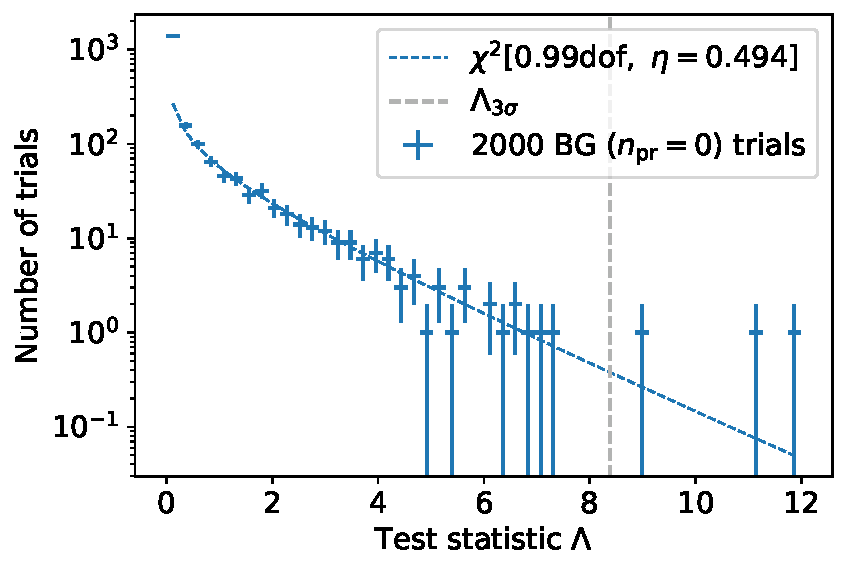
\includegraphics[width=0.49\textwidth]{../Plots/background_distribution_fit_conv=1.pdf}
    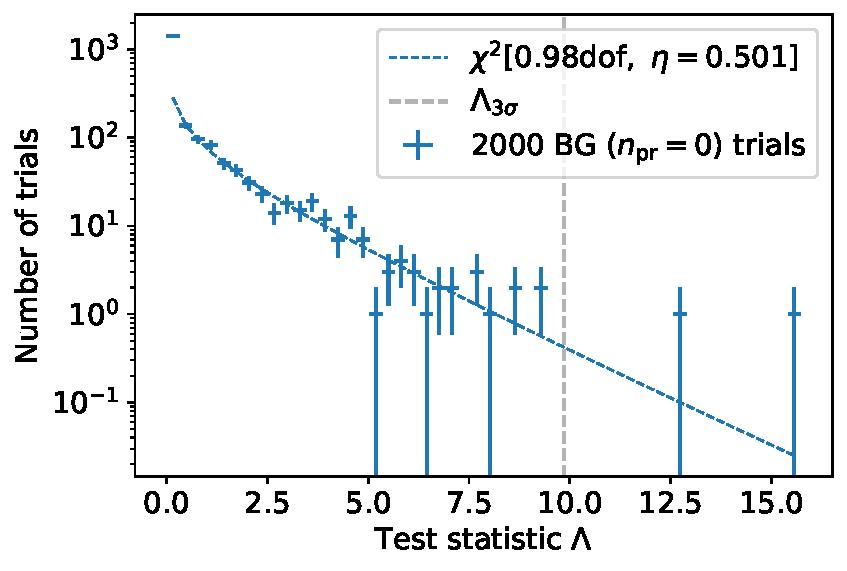
\includegraphics[width=0.49\textwidth]{../Plots/background_distribution_fit_conv=10.pdf}
    \caption{left: injected conv norm $1$ ($5\sigma=23.38$), right: injected conv norm $10$ ($5\sigma=27.46$)}
  \end{figure}
\end{frame}
\begin{frame}
  \frametitle{Impact of binning}
  \begin{minipage}{0.49\textwidth}
    \begin{figure}
      \centering
      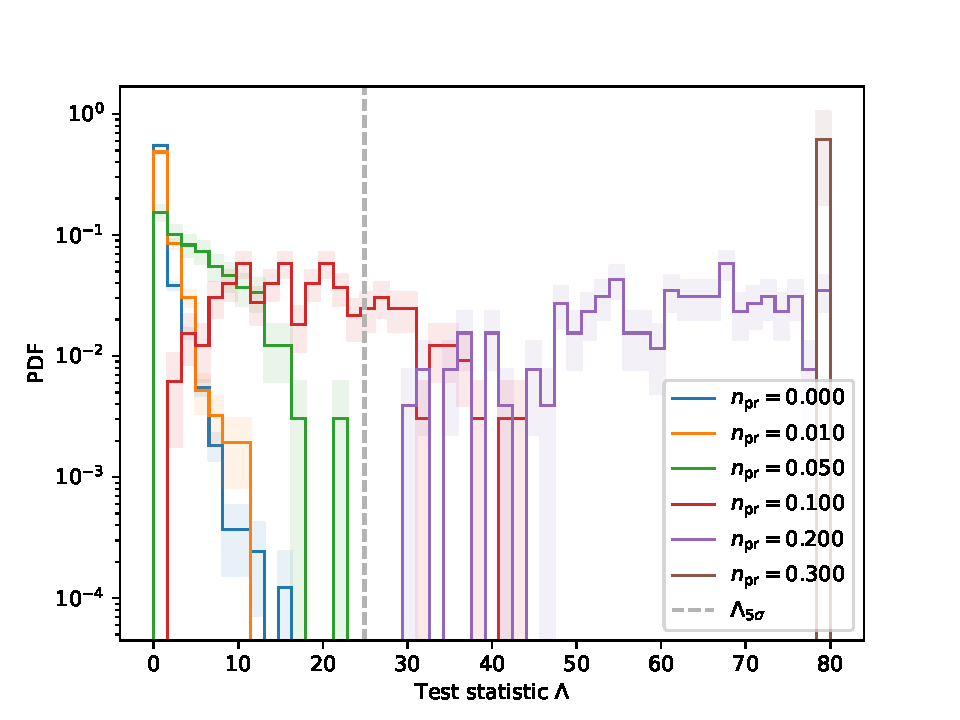
\includegraphics[width=0.85\textwidth]{../Plots/TS_Distribution_5e5_5bins}
      %\includegraphics[width=0.85\textwidth]{}
    \end{figure}
  \end{minipage}
  \begin{minipage}{0.49\textwidth}
    \begin{figure}
      \centering
      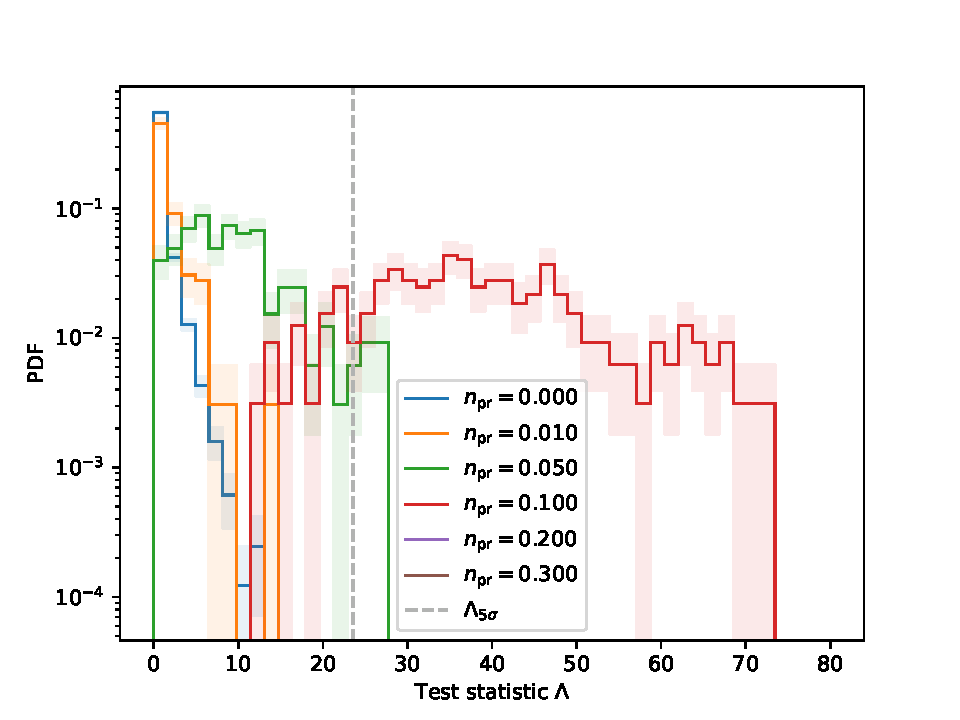
\includegraphics[width=0.85\textwidth]{../Plots/TS_Distribution_5e5_6bins}
      %\includegraphics[width=0.85\textwidth]{}
    \end{figure}
  \end{minipage}
\end{frame}
\end{document}